\documentclass[11pt, a4paper]{article}
\usepackage{amssymb}
\usepackage{amsmath}
\usepackage{graphicx}
\usepackage{float}
\usepackage{pdfpages}

\title{\textbf{GenGPT: A Package to Generate Synthetic Goal-Plan Trees}}
\begin{document}
\author{Yuan Yao\\[5mm]
School of Computer Science\\
University of Nottingham\\
yvy@cs.nott.ac.uk}
\date{}
\maketitle

GenGPT is a package to generate synthetic goal-plan trees \cite{conf/ijcai/thangarajah03,journal/jar/thangarajah11}. Goal-plan trees are widely used in BDI-based agent programming to represent the relations between goals, plans and actions, and to reason about the interactions between intentions. The root of a goal-plan tree is a (top-level) goal (goal-node), and its children are the plans that can be used to achieve the goal (plan-nodes). Plans may in turn contain primitive actions (action nodes) and subgoals (goal nodes), giving rise to a tree structure representing all possible ways an agent can achieve the top-level goal. 

GenGPT can be used in a standalone fashion using the bundled Java application to generate a set of goal-plan trees (in XML format) as input to another program. Alternatively, the source code provided can be integrated directly into another program. Note that GenGPT is licensed under the GNU Public License (GPL) Version 3. See the file \texttt{LICENSE.txt} for details.

Section \ref{sec:running-GenGPT} below describes the  characteristics of the synthetic goal-plan trees generated by GenGPT, and explains how to generate sets of tress using the GenGPT java application. Section \ref{sec:code} briefly describes the organisation of the code.

\section{Running the GenGPT Application}
\label{sec:running-GenGPT}

The application is packaged as a jar file, and is invoked from the command-line as

\vspace{3mm}
\texttt{java -jar GenGPT.jar <args>}

\vspace{3mm}
The arguments required to generate the set of goal-plan trees are: the depth of the goal-plan tree $\#\delta$, the number of subgoals in each non-leaf plan (leaf plans contain only action nodes) $\#\gamma$, the number of plans to achieve a goal $\#\pi$, the number of actions in each plan $\#\alpha$, 
% This is a bit awkward, but I can't think of another form of words; you can't say 'executed in parallel' since a goal-plan tree is not executed.
the probability that actions and subgoals in a plan form part of a parallel composition $\rho$, the number of environment variables that may appear in the tree as pre-, in-, and postconditions $\#\nu$, the number of goal-plan trees $\#T$ and the output file path $Path$ to which the forest of goal-plan trees is saved. The flag for each argument, their default values and the constraints on each argument are shown in Table \ref{arguments}.

\begin{table}[h!]
\centering
\caption{Arguments required to generate the goal-plan trees}
\label{arguments}
\begin{tabular}{|l|l|l|l|l|}
\hline
Symbol & Flag & Default & Constraints& Description \\ \hline\hline
$\#\delta$ & -d & 3 & $\#\delta\geq$ 1 & depth of the tree \\ \hline
$\#\gamma$ & -g & 1 & $\#\gamma\geq$ 1& number of subgoals in each plan  \\ \hline
$\#\pi$ &  -p & 2 & $\#\pi \geq$ 1& number of plans to achieve a goal \\ \hline
$\#\alpha$ & -a & 1 & $\#\alpha \geq$ 1& number of actions in each plan  \\ \hline
$\rho$ & -l & 0 &$1 \geq \rho \geq 0$ & probability of parallel execution  \\ \hline
$\#\nu$& -v & 50 & $\#\nu \geq$ 1& number of environment variables \\ \hline
$\#T$ & -t & 1 & $\#T \geq$ 1& number of goal-plan trees \\ \hline
$Path$ & -f & gpt.xml & \ & output file path\\  \hline
\end{tabular}
\end{table}

The arguments $\#\delta$, $\#\gamma$, $\#\pi$ and $\#\alpha$ together determine the shape of the goal-plan trees in the forest.\footnote{It would be more flexible to allow  specification of the maximum and minimum number of actions and subgoals in each plan; we assume a fixed number of actions and subgoals for simplicity.} By default, the actions and subgoals in each plan are executed sequentially. The parameter $\rho$ specifies the probability that a plan will be generated in which the actions and subgoals are executed in parallel. $\#\nu$ represents the number of variables that may appear in each goal-plan tree (as the pre- and post-conditions of actions and plans). By varying the value of $\#\nu$ we can vary the likelihood of actions and plans in different goal-plan trees having the same pre- and postconditions, and hence the probability of both positive and negative interactions between goal-plan trees.

The set of goal-plan trees is saved in XML format. The BNF for the XML format is shown in Figure \ref{fig:xml}. 
%
The XML file contains a forest of goal-plan trees. Each goal  $\gamma$ has a set of plans $\pi_1, \ldots, \pi_n$ to achieve it. Each plan $\pi$ consists of a sequence of actions and subgoals, $\pi = \alpha_1 ; \ldots ; \alpha_m$, or a parallel composition of actions and subgoals, $\pi = \alpha_1 \| \ldots \| \alpha_m$, where each $\alpha_i$ is either an action or a subgoal. We model the environment as a set of propositional variables, and define pre, in- and postconditions as a set of literals. Each literal is denoted by an $(index, boolean)$ pair in the XML file, where $integer$ is an identifier of the propositions and $boolean$ is either true or false.
%
An example goal-plan tree generated by GenGPT with parameters $\#\delta$ = 5, $\#\gamma$ = 1, $\#\pi$ = 2, $\#\alpha$ = 3, $\rho$ = 0, $\#\nu$ = 100, $\#T$ = 1, $Path$ = example-gpt.xml is shown in Figure \ref{fig:gpt}), and the XML can be found in the file \texttt{example-gpt.xml}.

\begin{figure}[!h]
\centering\small
\begin{tabular}{ r c l }
  $\langle$Forest$\rangle$ & $::=$ & $\langle$Goal$\rangle$ (, $\langle$Goal$\rangle$$)^*$\\
  $\langle$Goal$\rangle$ & $::=$ & $\langle$Name$\rangle$ $\langle$Incondition$\rangle$ $\langle$Plans$\rangle$  \\
  $\langle$Plans$\rangle$ & $::=$ & $\langle$Plan$\rangle$ (, $\langle$Plan$\rangle$$)^*$ \\
  $\langle$Plan$\rangle$ & $::=$ & $\langle$Name$\rangle$  $\langle$Precondition$\rangle$ $\langle$Incondition$\rangle$ $\setlength{\tabcolsep}{5pt}\langle$PlanBody$\rangle$\\
  $\langle$PlanBody$\rangle$ & $::=$ & $\langle$Step$\rangle$ ( (; $\langle$Step$\rangle$$)^*$ $|$ $(\|$ $\langle$Step$\rangle$$)^+$ ) \\
   $\langle$Action$\rangle$ & $::=$ & $\langle$Name$\rangle$ $\langle$Precondition$\rangle$ $\langle$Incondition$\rangle$ $\langle$Postcondition$\rangle$ \\

&& \\
  $\langle$Precondition$\rangle$ & $::=$ & \textbf{$\epsilon$} $|$ $\langle$Literal$\rangle$\\
 $\langle$Incondition$\rangle$ & $::=$ & \textbf{$\epsilon$} $|$ $\langle$Literal$\rangle$ \\
  $\langle$Postcondition$\rangle$ & $::=$ & \textbf{$\epsilon$} $|$ $\langle$Literal$\rangle$ \\
  $\langle$Literal$\rangle$ & $::=$ &  ($\langle$Variable$\rangle$ , $\langle$Value$\rangle$) \\
  $\langle$Variable$\rangle$ & $::=$ & \textit{Integer}  \\
  $\langle$Value$\rangle$ & $::=$ & \textit{Boolean} \\
\end{tabular}
%\setlength{\belowcaptionskip}{-12pt}
\caption{XML format in which goal-plan trees are saved}
\label{fig:xml}
\end{figure}

\begin{figure}[!h]
\centering
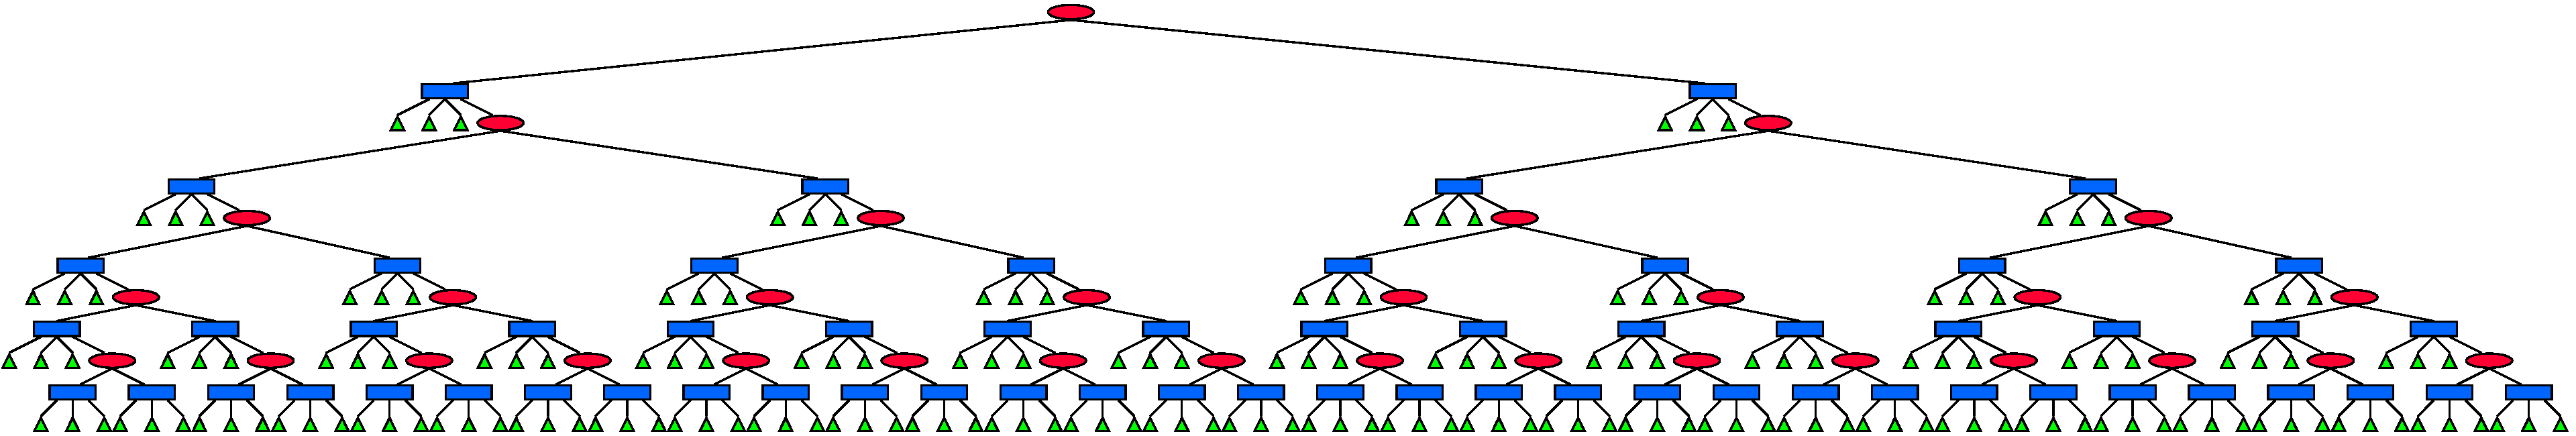
\includegraphics[width=1\textwidth]{example-gpt}
\caption{Example goal-plan tree.}
\label{fig:gpt}
\end{figure}



\section{The Code}
\label{sec:code}

The code consists of two main packages.
%\texttt{uno.gpt.nodes} and \texttt{uno.gpt.generator}. 
The package \texttt{uno.gpt.nodes} contains classes representing the tree nodes (i.e., goal nodes, plan nodes, action nodes and parallel composition nodes) and literals. The package \texttt{uno.gpt.generator} contains the class \texttt{Generator} which generates a forest of goal-plan trees, and the class \texttt{XMLWriter} which saves the forest in an XML file. In the remainder of this section, we focus on the tree generation code and briefly explain the rationale underlying tree generation.

A \textit{Literal} is defined as a tuple $(index, boolean)$, where $0 \leq index \leq \#\nu -1$ (where $\#\nu$ is the number of environment variables), and $boolean$ is either $True$ or  $False$. Goals, plans, actions and parallel compositions are represented using the java classes \texttt{GoalNode}, \texttt{PlanNode}, \texttt{ActionNode} and  \texttt{ParallelNode} respectively. Each \texttt{GoalNode} consists of a name, an in-condition and a list of \texttt{PlanNodes} representing plans which achieve the goal. Each \texttt{PlanNode} consists of a name, a pre-condition, an in-condition, and a list of nodes representing plan steps, which may be \texttt{GoalNodes}, \texttt{ActionNodes} or \texttt{ParallelNodes}. Each \texttt{ActionNode} consists of a name, together with the pre-, in- and postconditions of the action. Finally, each \texttt{ParallelNode} consists of a list of \texttt{ActionNodes} and \texttt{GoalNodes} to be executed in parallel.

The method \texttt{genTopLevelGoal} of the class \texttt{Generator} is used to iteratively generate goals, plans, and actions from the top-level goal to the leaf nodes in the tree. It first generates the top-level goal, and then calls the method \texttt{constructGoal} to generate the plans to achieve the top-level goal, and then generates either a sequence of actions and subgoals or a parallel composition for each of these plans and so on. 
%
The method \texttt{constructGoal} is used to generate plans to achieve a target goal and takes 4 parameters as arguments which are the target goal (\texttt{gl}), the depth of the target goal (\texttt{currentdepth}), the set of literals which can be selected as the precondition of the plans to achieve the target goal (\texttt{var\char`_pre}) and the set of literals which can be selected as the postcondition of the actions in the plans to achieve the target goal (\texttt{var\char`_post}). 
%
To generate plans for a top-level goal, \texttt{gl} is set to be the top-level goal, \texttt{currentdepth} is 1, \texttt{var\char`_pre} is empty and \texttt{var\char`_post} contains all possible literals. 
%
For each target goal, $\#\pi$ plans are generated. If \texttt{var\char`_pre} is not empty, the precondition of each plan is randomly selected from \texttt{var\char`_pre}. Otherwise, a proposition $i$ is randomly selected from the set of environment variables, where $i$ is an index. The odd numbered plans to achieve the goal have the literal $(i, \mathit{True})$ as their precondition, and the even numbered plans have $(i, \mathit{False})$ as their precondition. This ensures that if $\#\pi > 1$, there is at least one plan applicable to achieve each (sub)goal. 

%As mentioned, a plan may consist of a sequence of actions and subgoals or a parallel composition of action and subgoals. 
As explained above, with probability 1-$\rho$ a plan consists of an ordered sequence of actions and subgoals, and with probability $\rho$, it consists of a parallel composition of actions and subgoals.
%
If a plan consists of an ordered sequence of actions and subgoals, the method \texttt{constructPlan} is called to create the actions and subgoals in it. The \texttt{constructPlan} method takes 4 variables as its input, which are the target plan (\texttt{pl}), the depth of the target plan in the goal-plan tree (\texttt{currentdepth}), the set of literals which can be selected as the precondition of the plans to achieve the subgoals in the target plan (\texttt{var\char`_pre}) and the set of literals which can be selected as the postcondition of the actions in the target plan (\texttt{var\char`_post}). 
%
(The parameters \texttt{currentdepth}, \texttt{var\char`_pre}, \texttt{var\char`_post} are the same as in the method \texttt{constructGoal}.)
%
The actions in the plan are generated before the subgoals. 
%
The field \texttt{action\char`_pre}  is used to represent the set of literals that can be used as the precondition of the action. 
When generating the first action in the plan, \texttt{action\char`_pre} only contains the plan's precondition. Thus, the first action in each plan always has the plan's precondition as its own precondition. We then generate the postcondition of the action by randomly selecting a literal $l$ from \texttt{var\char`_post}. The sets of literals \texttt{action\char`_pre} and \texttt{var\char`_pre} are then updated as follows:

\begin{itemize}
\item if \texttt{action\char`_pre} (or \texttt{var\char`_pre}) contains the negation of $l$, remove the negation of $l$ from \texttt{action\char`_pre} (resp.\ \texttt{var\char`_pre}); 
\item if \texttt{action\char`_pre} (or \texttt{var\char`_pre}) doesn't contain $l$, add $l$ to \texttt{action\char`_pre} (resp.\ \texttt{var\char`_pre}).
\end{itemize} 
%
This updating process removes the literals which are made false by the new action from \texttt{action\char`_pre} and \texttt{var\char`_pre}, and adds the postcondition of the new action to both sets of literals.  The updated sets \texttt{action\char`_pre} and \texttt{var\char`_pre} are used for generating subsequent actions and subgoals. 

When all actions have been generated, if the plan is not a leaf plan (\texttt{currentdepth} != $\#\delta$), we also generate $\#\gamma$ subgoals. For each subgoal, the method \texttt{constructGoal} is called to add plans to achieve it. \texttt{gl} is the target subgoal, \texttt{currentdepth} is the current depth of the plan plus 1, and the other parameters are as in the method \texttt{constructPlan}. After generating each subgoal, we update the set of literals \texttt{var\char`_pre}. As subgoals may be achieved by different plans, we use the \textit{necessary postcondition} of the goal to present the set of literals that must be true after achieving this subgoal, and use \textit{contingent postcondition} to present the set of literals that may be true after achieving this subgoal \cite{Yao//:16b}. If the \textit{necessary postcondition} and \textit{contingent postcondition} of a subgoal are represented as $post_n$ and $post_c$ respectively, then the process of updating the literals in \texttt{var\char`_pre} is as follows:

\vspace{2mm}
\begin{tabular}{ l }
for each $l$ in $post_c$ do \\
\hspace{3mm}if \texttt{var\char`_pre} contains $\neg l$, remove $\neg l$ from \texttt{var\char`_pre} \\[2mm]

for each $l$ in $post_n$ do \\
\hspace{3mm}if \texttt{var\char`_pre} contains $\neg l$, remove $\neg l$ from \texttt{var\char`_pre} \\
\hspace{3mm}if \texttt{var\char`_pre} doesn't contain $l$, add $l$ to \texttt{var\char`_pre}\\
\end{tabular}

\vspace{2mm}

\noindent
This process removes the literals that are (necessarily or contingently) made false by achieving this goal from \texttt{var\char`_pre}, and adds the necessary postcondition of the goal to \texttt{var\char`_pre}. The updated \texttt{var\char`_pre} is then used to generate the subsequent subgoals in the plan. This process ensures the plan is executable if its precondition holds, and the choice of plans for the subgoal(s) in the plan is not affected by the postconditions of the actions in this plan.

If the plan consists of a parallel composition of actions and subgoals, the method  \texttt{constructParallelPlan} is used to create a parallel composition of actions and subgoals in the plan. As with the method \texttt{constructPlan}, it takes 4 parameters as its arguments, which are the target plan (\texttt{pl}), the depth of the target plan in the goal-plan tree (\texttt{currentdepth}), the set of literals which can be selected as the precondition of  plans to achieve subgoals in the target plan (\texttt{var\char`_pre}) and the set of literals which can be selected as the postcondition of the actions in the target plan (\texttt{var\char`_post}). 
%
The parameter \texttt{pl} is the plan whose plan body will be the new parallel composition, and the other three parameters are passed by the method \texttt{constructGoal}. If \texttt{pl} is a leaf plan, the parallel composition contains only $\#\alpha$ actions. Otherwise, the parallel composition contains $\#\alpha$ actions and $\#\gamma$ subgoals. 
%
Each action in the parallel composition has the plan's precondition as its precondition, and its postcondition, $l$, is randomly selected from \texttt{var\char`_post}. 
%
Once a postcondition $l$ is selected, $l$ and its negation are removed from \texttt{var\char`_post}, and thus cannot be used as the postcondition of all other actions in the same parallel composition. By doing so, we ensure the postcondition of actions in one parallel composition do not conflict with each other, and there are no identical actions in the parallel composition (i.e., actions which have same precondition and postcondition).
%
For the subgoals in the parallel composition, we divide the set of literals that can be selected as the postcondition of the actions in the plan(s) for a subgoal into $\#\gamma$ subsets. Each subset contains the same number of distinct variables, and is denoted as \texttt{var\char`_post$_i$} where $0 \leq i \leq \#\gamma - 1$.
%
For each subgoal in the parallel composition, the method \texttt{constructGoal} is called to add plans to achieve the goal. The parameter \texttt{gl} of \texttt{constructGoal} is the subgoal for which plans must be generated, the parameter \texttt{currentdepth} is incremented to be the current depth of the plan containing the parallel composition plus 1, the parameter \texttt{var\char`_pre} is set to contain only the precondition of the plan containing the subgoal gl (i.e., whose plan body is the parallel composition containing gl),
%
and finally the parameter \texttt{var\char`_post} is set to be \texttt{var\char`_post$_i$} if \texttt{gl} is the ${i+1}^{th}$ subgoal in the parallel composition.
%
The whole process of generating parallel composition ensures that there are no potential conflict between these actions and subgoals and the overall postcondition of the plan is ``stable''.

We keep creating actions, plans, (sub)goals and parallel compositions until we reach the depth of the tree. The generation process will stop after we generate the last leaf action, and the whole goal-plan tree is translated and saved in an XML file by using the method in the java class \texttt{XMLWriter}. 

% This is irrelevant.
%As different agent programming language may require different ``parsers'' (i.e., to read the goal-plan trees from the XML file), we didn't provide any parser to read the XML file in the current application.

% This would be better earlier, when you introduce the idea of a goal-plan tree.
%Figure \ref{fig:gpt} shows a goal-plan tree with $\delta$ = 5, $\#\gamma$ =1, $\#\pi$ = 2, $\#\alpha$ = 3, $\rho$ = 0, where goals are in red, plans are in blue and actions are in green

%\begin{figure}[!h]
%\centering
%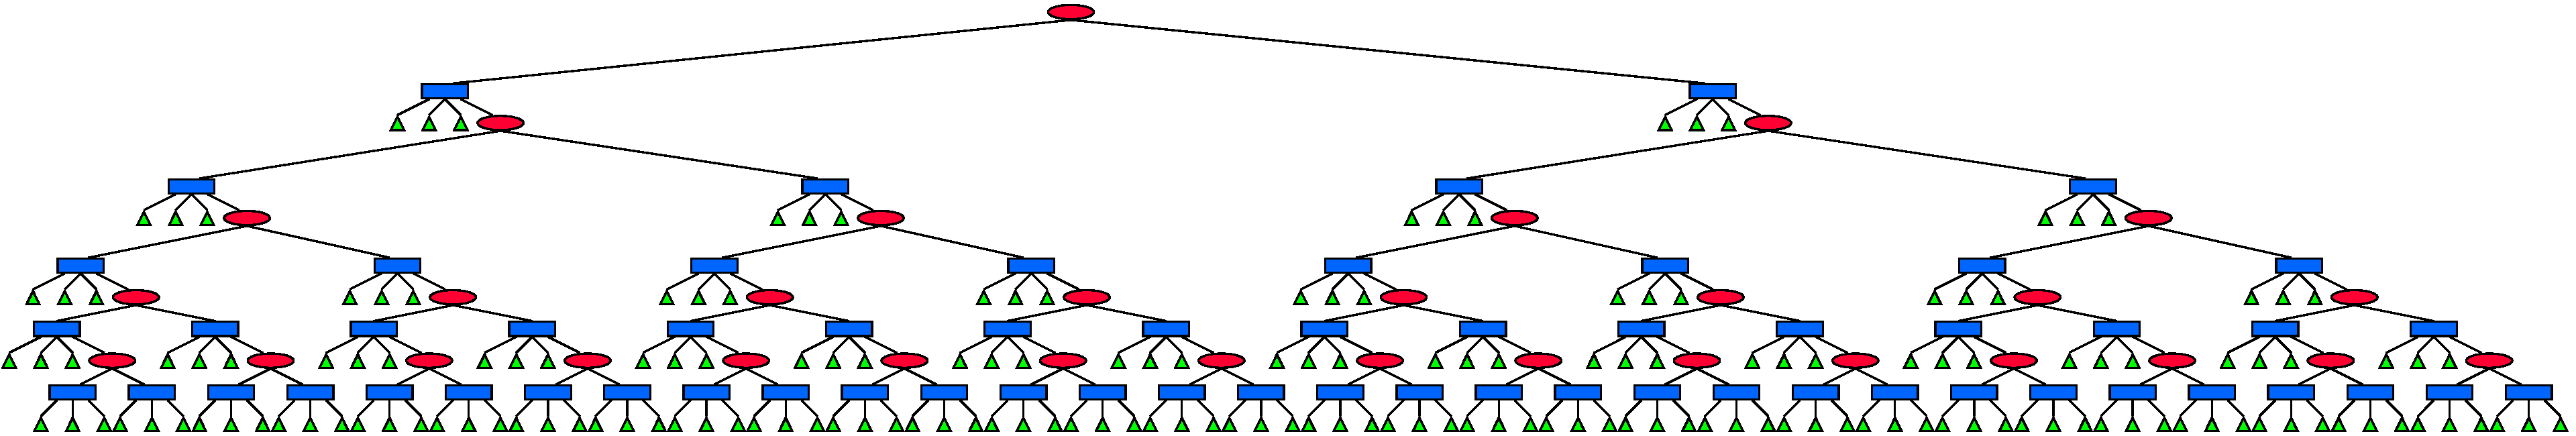
\includegraphics[width=1\textwidth]{example-gpt}
%\caption{Synthetic goal-plan tree.}
%\label{fig:gpt}
%\end{figure}


\bibliographystyle{abbrv}
%\bibliography{aamas16-mcts}
\begin{thebibliography}{10}

\bibitem{conf/ijcai/thangarajah03}
J.~Thangarajah, L.~Padgham, and M.~Winikoff.
\newblock Detecting {\&} avoiding interference between goals in intelligent
  agents.
\newblock In G.~Gottlob and T.~Walsh, editors, {\em Proceedings of the
  Eighteenth International Joint Conference on Artificial Intelligence
  ({IJCAI}-03)}, pages 721--726, Acapulco, Mexico, August 2003. Morgan
  Kaufmann.

\bibitem{journal/jar/thangarajah11}
J.~Thangarajah and L.~Padgham.
\newblock Computationally effective reasoning about goal interactions.
\newblock {\em Journal of Automated Reasoning}, 47(1):17--56, 2011.

\bibitem{Yao//:16b}
Yuan Yao, Lavindra de Silva, and Brian Logan.
\newblock Reasoning about the Executability of Goal-Plan Trees
\newblock Proceedings of the Fourth International Workshop on Engineering Multi-Agent Systems, 2016.
\end{thebibliography}

\end{document}